\documentclass[aspectratio=169]{beamer}

\usepackage[utf8]{inputenc}
\usepackage{times}
\usepackage{mathptmx}

\usepackage{graphicx}
\usepackage[outdir=./figs/]{epstopdf}
\graphicspath{ {./figs/} }


%%%%% definición de colores para el tema
\usetheme{Madrid}
\useoutertheme{infolines} % Alternatively: miniframes, infolines, split
\useinnertheme{circles}

\definecolor{nordwhite}{rgb}{0.9255, 0.9373, 0.9569}
\definecolor{nordgrey}{rgb}{0.298, 0.3373, 0.4157}
\definecolor{nordblue}{rgb}{0.3686, 0.5059, 0.6745} % nord blue (primary)
\definecolor{nordlblue}{rgb}{0.5059, 0.6314, 0.7569}
\definecolor{nordllblue}{rgb}{0.5333, 0.752, 0.8157} % nord lblue (secondary)
\definecolor{nordlllblue}{rgb}{0.5608, 0.7373, 0.7333}

\setbeamercolor{background canvas}{bg=nordwhite}
\setbeamercolor{normal text}{fg=nordgrey}

\setbeamercolor{palette primary}{bg=nordblue,fg=nordwhite}
\setbeamercolor{palette secondary}{bg=nordlblue,fg=nordwhite}
\setbeamercolor{palette tertiary}{bg=nordllblue,fg=nordwhite}
\setbeamercolor{palette quaternary}{bg=nordlllblue,fg=nordwhite}

\setbeamercolor{structure}{fg=nordblue} % itemize, enumerate, etc
\setbeamercolor{section in toc}{fg=nordblue} % TOC sections

% Override palette coloring with secondary
\setbeamercolor{subsection in head/foot}{bg=nordlblue,fg=nordwhite}

% textbf con otro color
\let\oldtextbf\textbf
\renewcommand{\textbf}[1]{\textcolor{nordblue}{\oldtextbf{#1}}}

%%%%% caratula
\title[Potenciales de ML]{Potenciales interatómicos de aprendizaje automático y 
su aplicación a baterias de litio}
\subtitle{Seminario de doctorado}
\author[Francisco FERNANDEZ]{Francisco FERNANDEZ}
\logo{
    
\includegraphics[width=1.3cm,keepaspectratio]{logo_famaf.png}
}
\institute[FaMAF (UNC)]{Facultad de Matemática, Astronomía, Física y Computación 
(Universidad Nacional de Córdoba) \\ \scalebox{1.5}{\insertlogo}}
\date[\today]{\today}

% tabla de contenidos
\AtBeginSection[]
{
	\begin{frame}
		\frametitle{Índice}
		\tableofcontents[currentsection]
	\end{frame}
}

\begin{document}

    \frame{\titlepage}
	
	\begin{frame}
        \frametitle{Índice}
		\tableofcontents
	\end{frame}

    %%%% INTRODUCCION %%%%
    \section{Introducción}
    
    \begin{frame}
        \frametitle{Introducción}

        \begin{columns}
            \column{0.5\textwidth}
            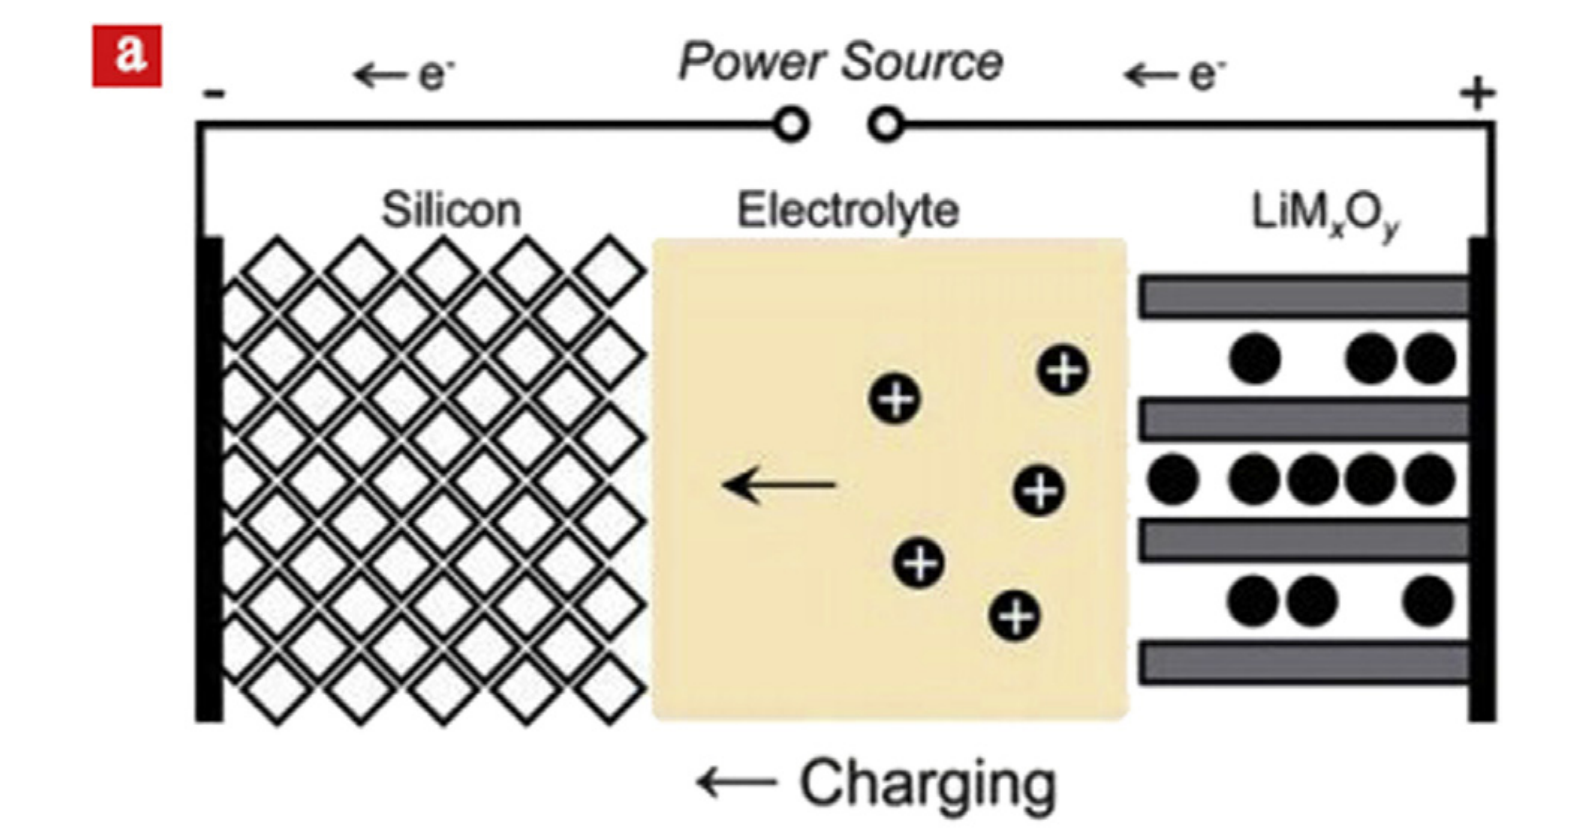
\includegraphics[width=\columnwidth]{intro-bateria-carga.png}
            \pause
            \column{0.5\textwidth}
            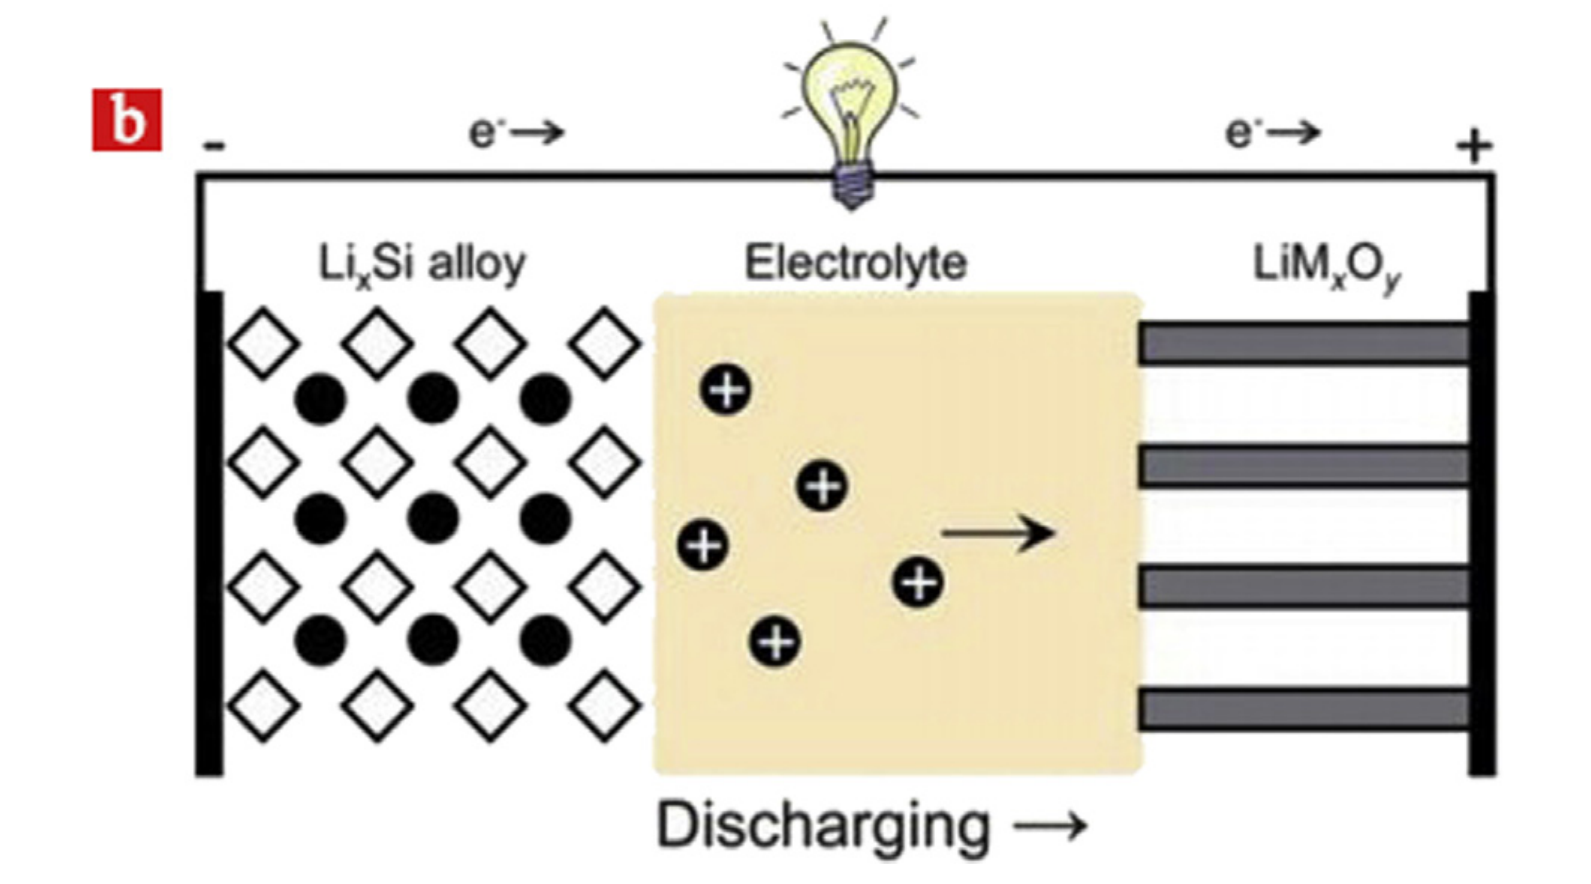
\includegraphics[width=\columnwidth]{intro-bateria-descarga.png}
        \end{columns}

	\end{frame}
    
    \begin{frame}
        \frametitle{Introducción}
        
        Para complementar la gran cantidad de \textbf{herramientas experimentales}
        (difracción de rayos x o neutrones, microscopía electrónica, resonancia
        magnética nuclear, espectroscopía de rayos x, etc) que existen para 
        estudiar materiales relevantes para las distintas partes de las baterias 
        se han venido realizando \textbf{simulaciones computacionales}, 
        principalmente:
        \begin{enumerate}
            \item Teoría del funcional de la densidad (DFT),
            \item campos de fuerzas (FF) en MD, MC, kMC, etc.
        \end{enumerate}

        \ \pause

        En este seminario se presenta un modelado emergente y complementario, los
        \textbf{potenciales interatómicos de aprendizaje automático} creados a 
        partir de datos de referencia provenientes de mecánica cuántica que buscan
        tener eficiencia y precisión cercanas a las de los FF y de DFT, 
        respectivamente.

	\end{frame}

    \begin{frame}
        \frametitle{Introducción}

        En la aproximación de Born-Oppenheimer, donde los núcleos de los átomos
        son considerados como partículas clásicas a la hora de determinar la 
        función de onda electrónica, la energía de un estado electrónico a partir 
        de las posiciones de los núcleos se conoce como la \textbf{superficie 
        energía-potencial (PES)} y está completamente definido por su Hamiltoniano
        electrónico.

        \pause

        \begin{center}
            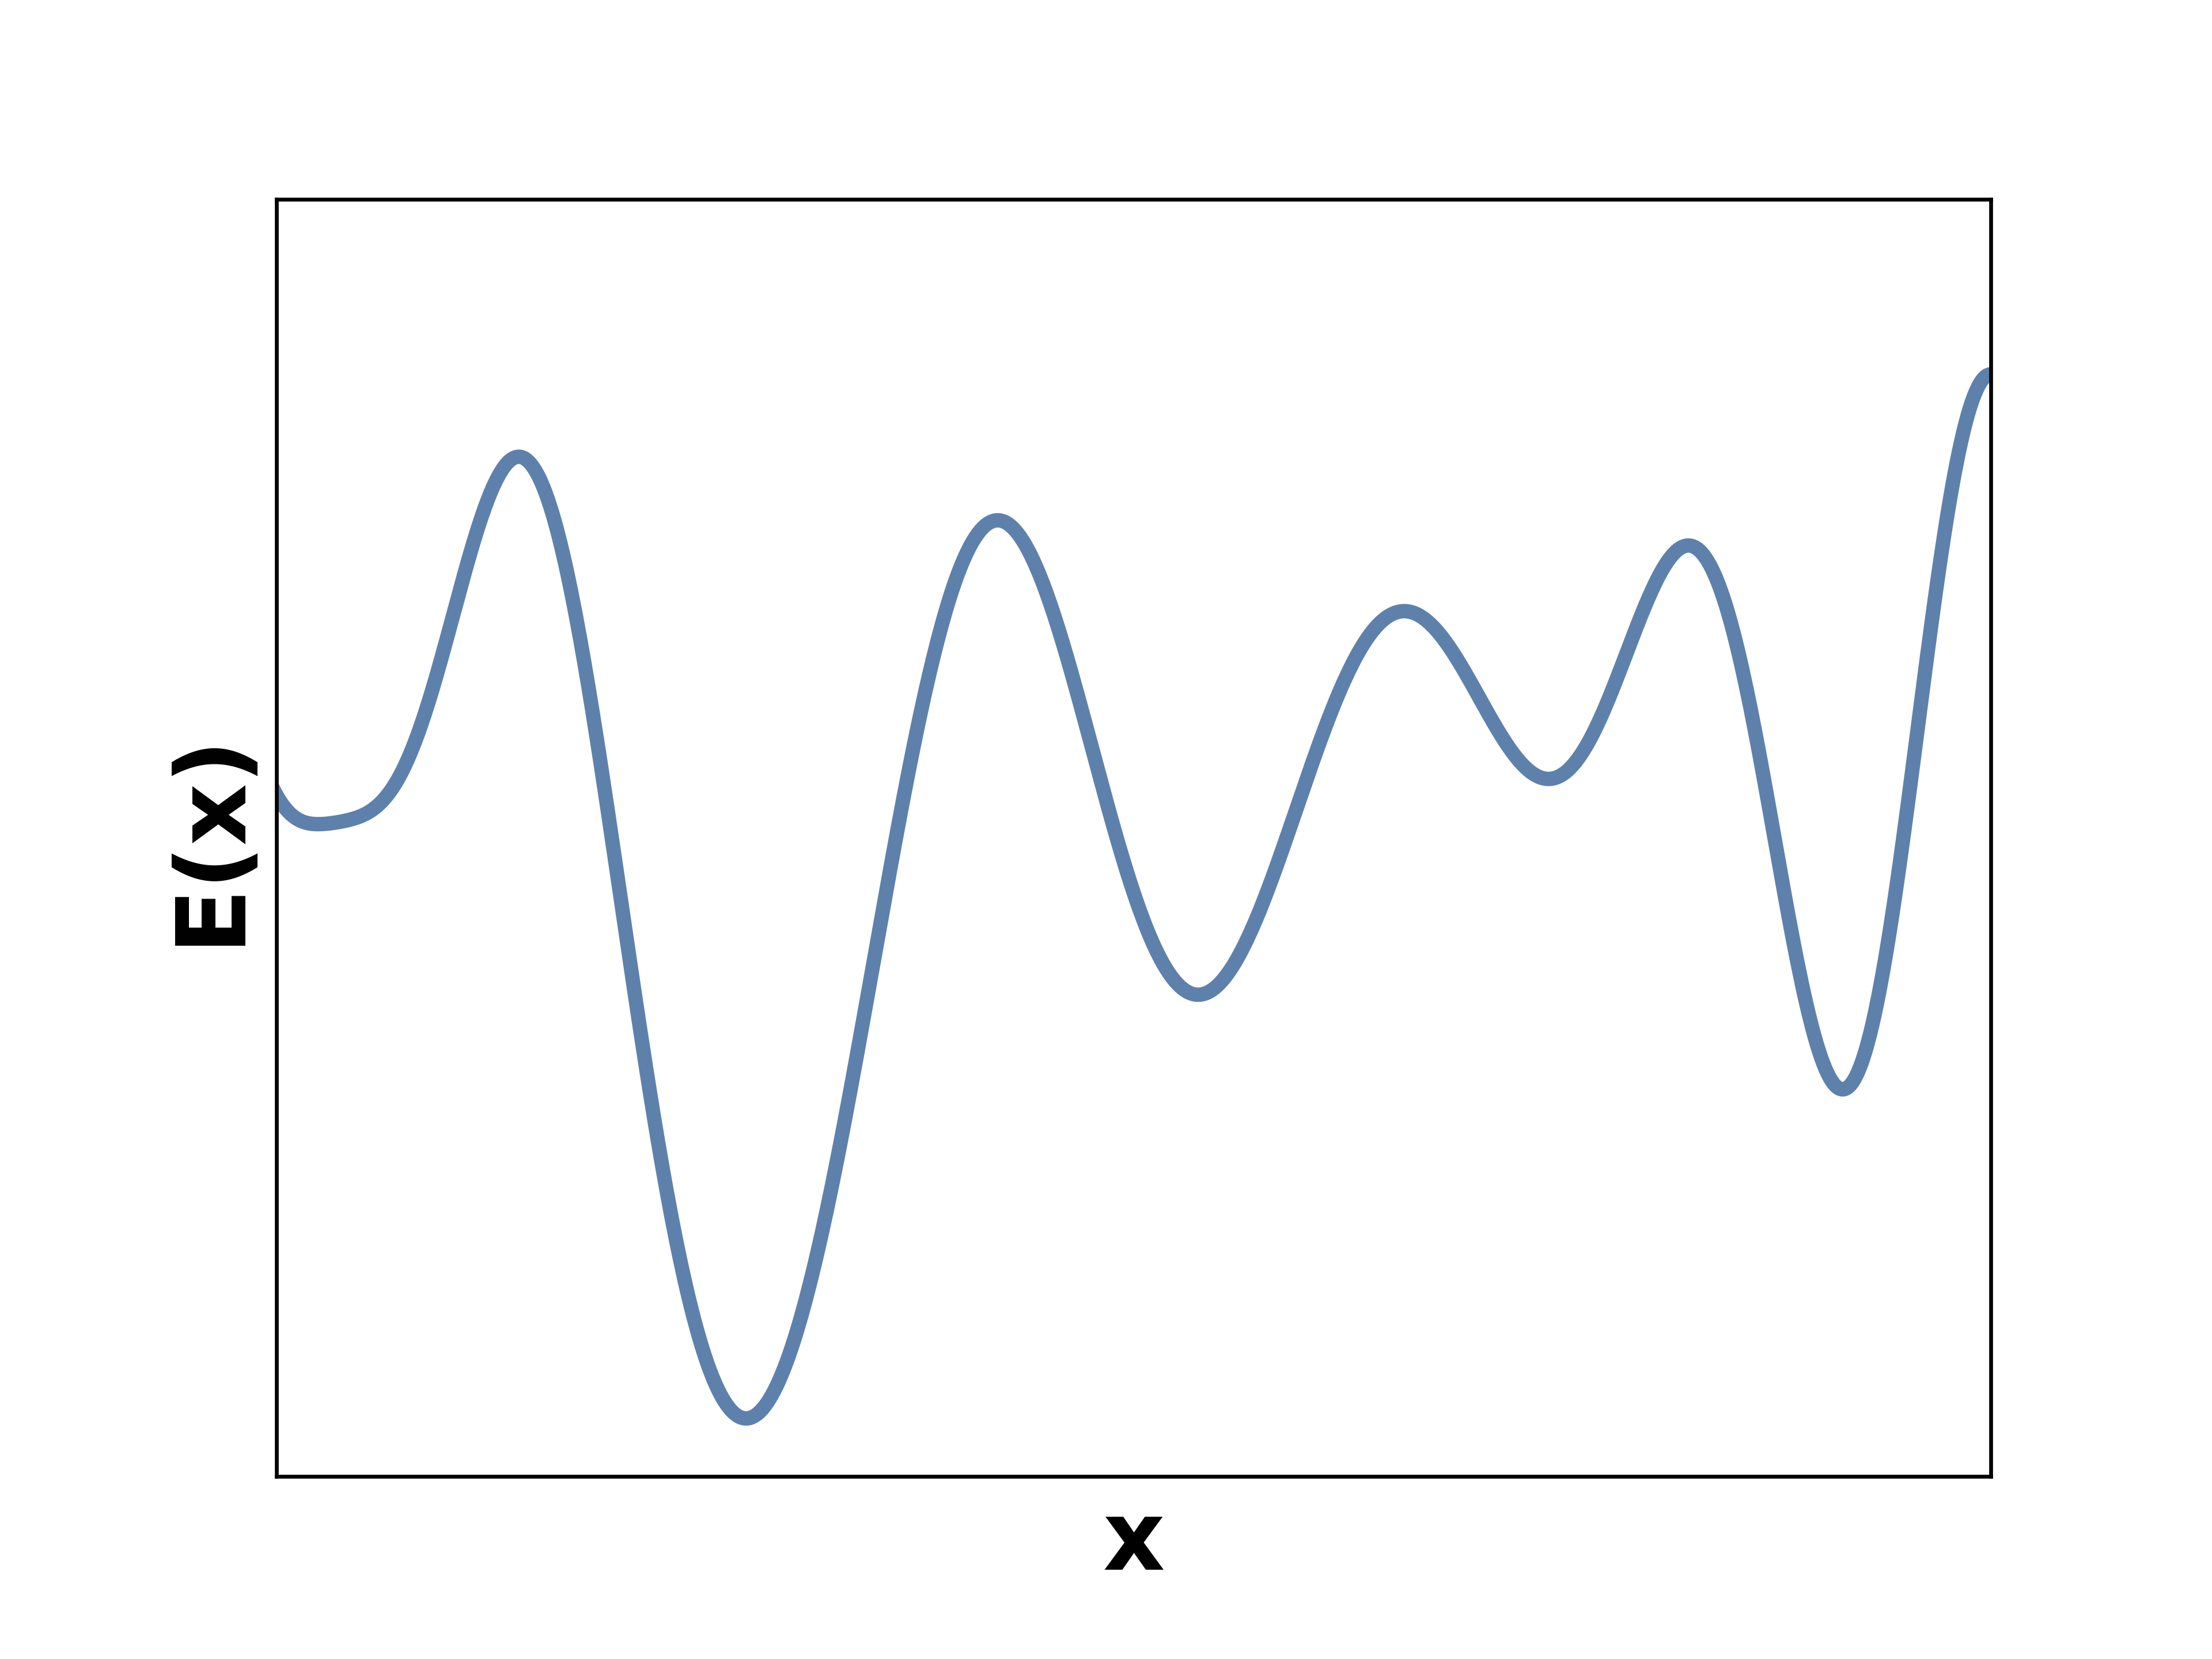
\includegraphics[width=0.35\textwidth]{intro-pes.png}
        \end{center}

	\end{frame}

    \subsection{Teoría del Funcional de la Densidad (DFT)}

	\begin{frame}
        \frametitle{Introducción: Teoría del Funcional de la Densiadad (DFT)}
        
        La forma más precisa de obtener distintos puntos de la \textbf{PES} 
        es a partir de cálculos de mecánica cuántica. Para estados estacionarios 
        tenemos que la ecuación de Schrödinger es 
        $$
        \hat{H} |\psi\rangle = E |\psi\rangle
        $$
        %$$
        %\hat{H} |\psi_n(t)\rangle = i\hbar\frac{\partial}{\partial t} |\psi_n(t)\rangle
        %$$
        \pause

        Para aproximar la solución a esta ecuación, uno de los métodos más 
        utilizados es la \textbf{Teoría del Funcional de la Densidad (DFT)}.

        \pause

        \begin{columns}
            \column{0.5\textwidth}
            \begin{itemize}
                \item Preciso.
            \end{itemize}

            \column{0.5\textwidth}
            \begin{itemize}
                \item Algunos cientos de átomos y tiempos menores al ns.
                \item Escalea al cubo de la cantidad de electrones.
            \end{itemize}
        \end{columns}
        
	\end{frame}
    
    \subsection{Potenciales interatómicos empíricos (FF)}
	
    \begin{frame}
        \frametitle{Introducción: Potenciales interatómicos empíricos (FF)}

        Una aproximación a la \textbf{PES} puede obtenerse a partir de potenciales
        interatómicos o campos de fuerza (\textit{force fields}, \textbf{FF}), que
        relacionan directamente, a través de una forma funcional, la configuración
        atómica con la energía:
        
        \pause

        \begin{columns}
            \column{0.5\textwidth}
            \begin{itemize}
                \item potencial de Coulomb,
                \item potencial de Lennard-Jones,
                \item método del átomo embebido (EAM),
                \item ReaxFF.
            \end{itemize}
            \column{0.5\textwidth}
            \begin{center}
                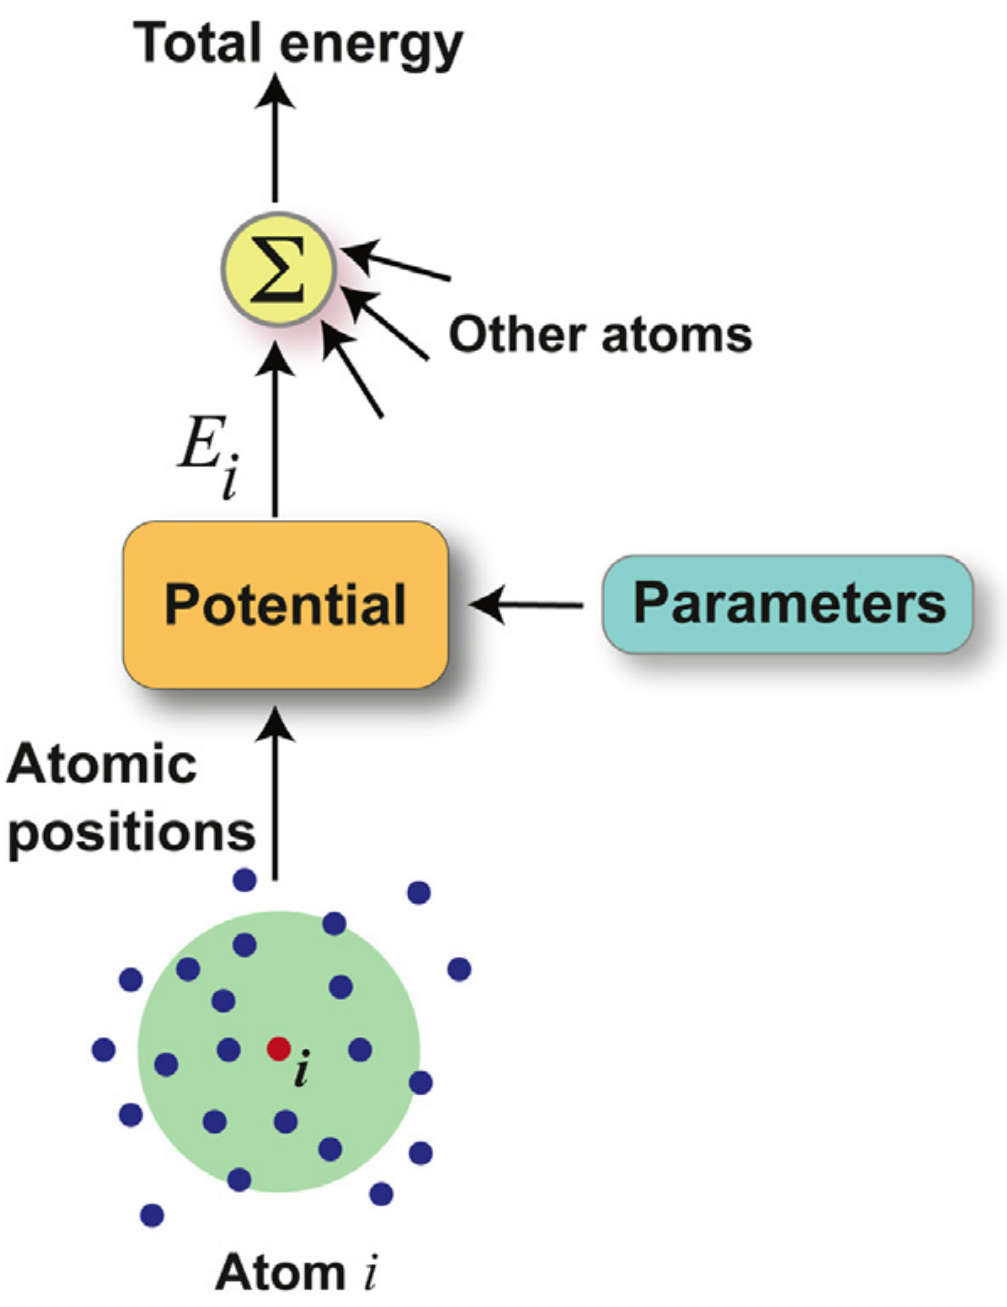
\includegraphics[width=0.45\columnwidth]{intro-ff.png}
            \end{center}
        \end{columns}

        \pause
        
        \begin{columns}
            \column{0.5\textwidth}
            \begin{itemize}
                \item Escalas de tiempo y tamaños más grandes que DFT.
            \end{itemize}

            \column{0.5\textwidth}
            \begin{itemize}
                \item Precisión limitada por la forma funcional.
            \end{itemize}
        \end{columns}

	\end{frame}
    
    \subsection{Potenciales interatómicos de aprendizaje automático (ML)}
    
    \begin{frame}
        \frametitle{Introducción: Potenciales interatómicos de aprendizaje 
        automático (ML)}

        \begin{center}
            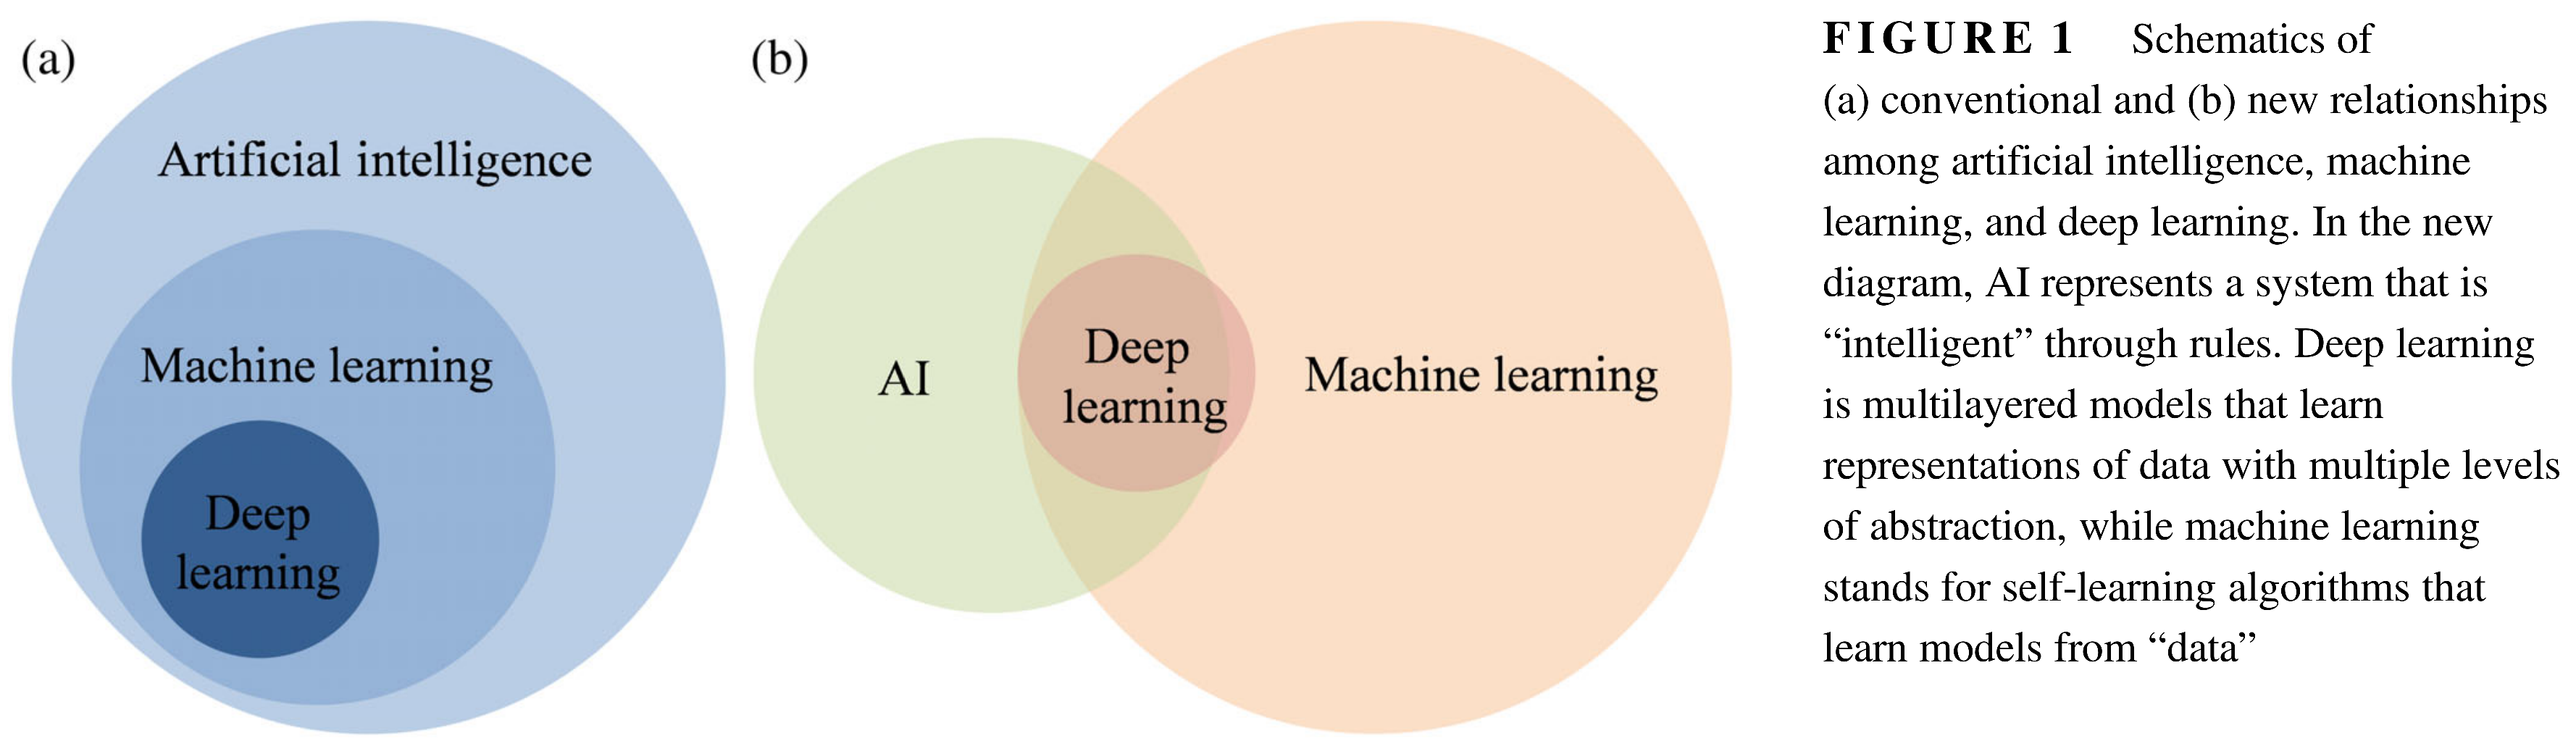
\includegraphics[width=0.7\textwidth]{intro-definicion-ML.png}
        \end{center}

        \pause
    
        En física, química, ciencias de los materiales, los métodos de ML se
        utilizan para buscar en grandes bases de datos relaciones ocultas entre 
        la estructura atómica y alguna propiedad de interés.

        \ \pause

        El tema de este seminario es la aplicación de algunos de estos métodos
        para ajustar la PES en función del entorno atómico.

	\end{frame}
	
    \begin{frame}
        \frametitle{Introducción: Potenciales interatómicos de aprendizaje 
        automático (ML)}

        En el aprendizaje automático supervisado el objetivo es identificar una
        función $f$ (\textit{potencial interatómico que se desea aprender}) que
        prediga valores $y$ (\textit{PES}) a partir de datos de entrada $x$ 
        (\textit{configuraciones de los átomos}).
        
        $$
        y = f(x)
        $$

        \pause

        \begin{center}
            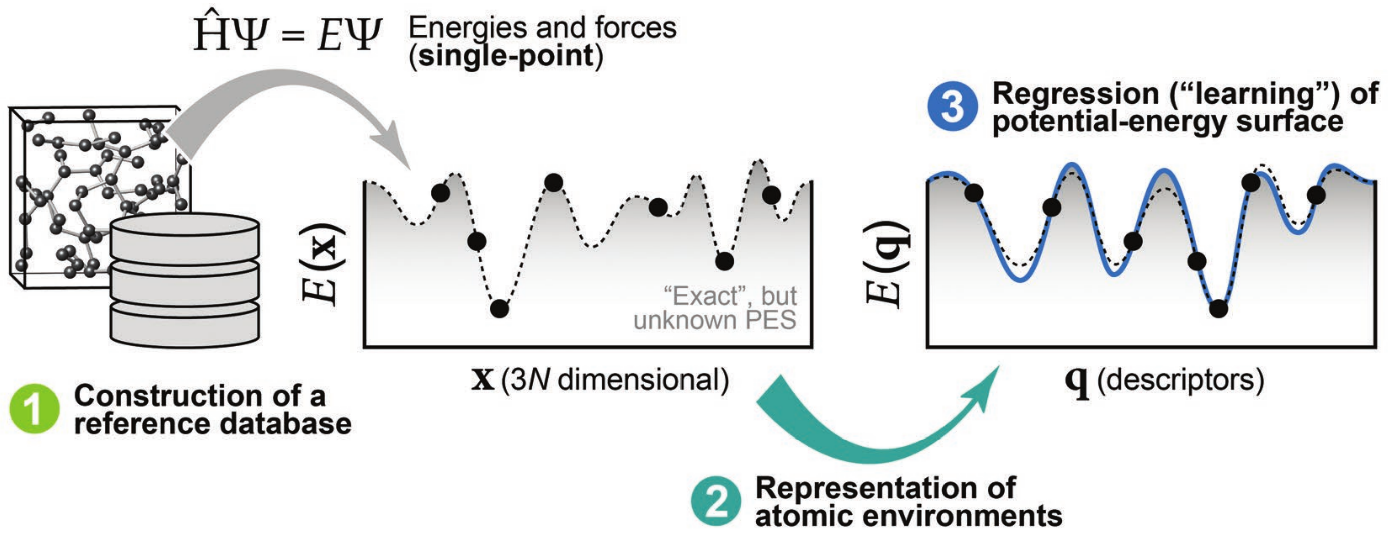
\includegraphics[width=0.75\textwidth]{intro-construccion.png}
        \end{center}

	\end{frame}
    
    \begin{frame}
        \frametitle{Introducción: Potenciales interatómicos de aprendizaje 
        automático (ML)}

        Los \textbf{potenciales interatómicos de aprendizaje automático} buscan
        combinar ambas ventajas de los FF (eficiencia) y de DFT (precisión).

        \ \pause

        Pueden definirse de la siguiente manera:
        \begin{itemize}
            \item Utiliza un método de ML para construir una relación funcional
                entre las configuraciones atómicas y su energía,
            \item no contienen aproximaciones físicas, a parte del método 
                utilizado para obtener los datos de referencia,
            \item se desarrolla utilizando un conjunto coherente de datos de
                estructura electrónica.
        \end{itemize}

	\end{frame}
    
    \begin{frame}
        \frametitle{Introducción: Potenciales interatómicos de aprendizaje 
        automático (ML)}

        Las posiciones atómicas necesitan ser transformadas a 
        \textbf{descriptores} adecuados para los \textbf{métodos de ML} que deben 
        cumplir con distintos \textit{constains} físicos:
        \begin{enumerate}
            \item Las contribuciones dominantes a la energía son de los átomos 
                más cercanos entre sí.
            \item La energía es invariante a permutaciones entre átomos del mismo 
                tipo, rotaciones, traslaciones.
            \item La PES varía suavemente con respecto a variaciones de las
                posiciones atómicas.
        \end{enumerate}

	\end{frame}
    
    \begin{frame}
        \frametitle{Introducción: Potenciales interatómicos de aprendizaje 
        automático (ML)}

        \begin{columns}
            \column{0.5\textwidth}
            \begin{center}
                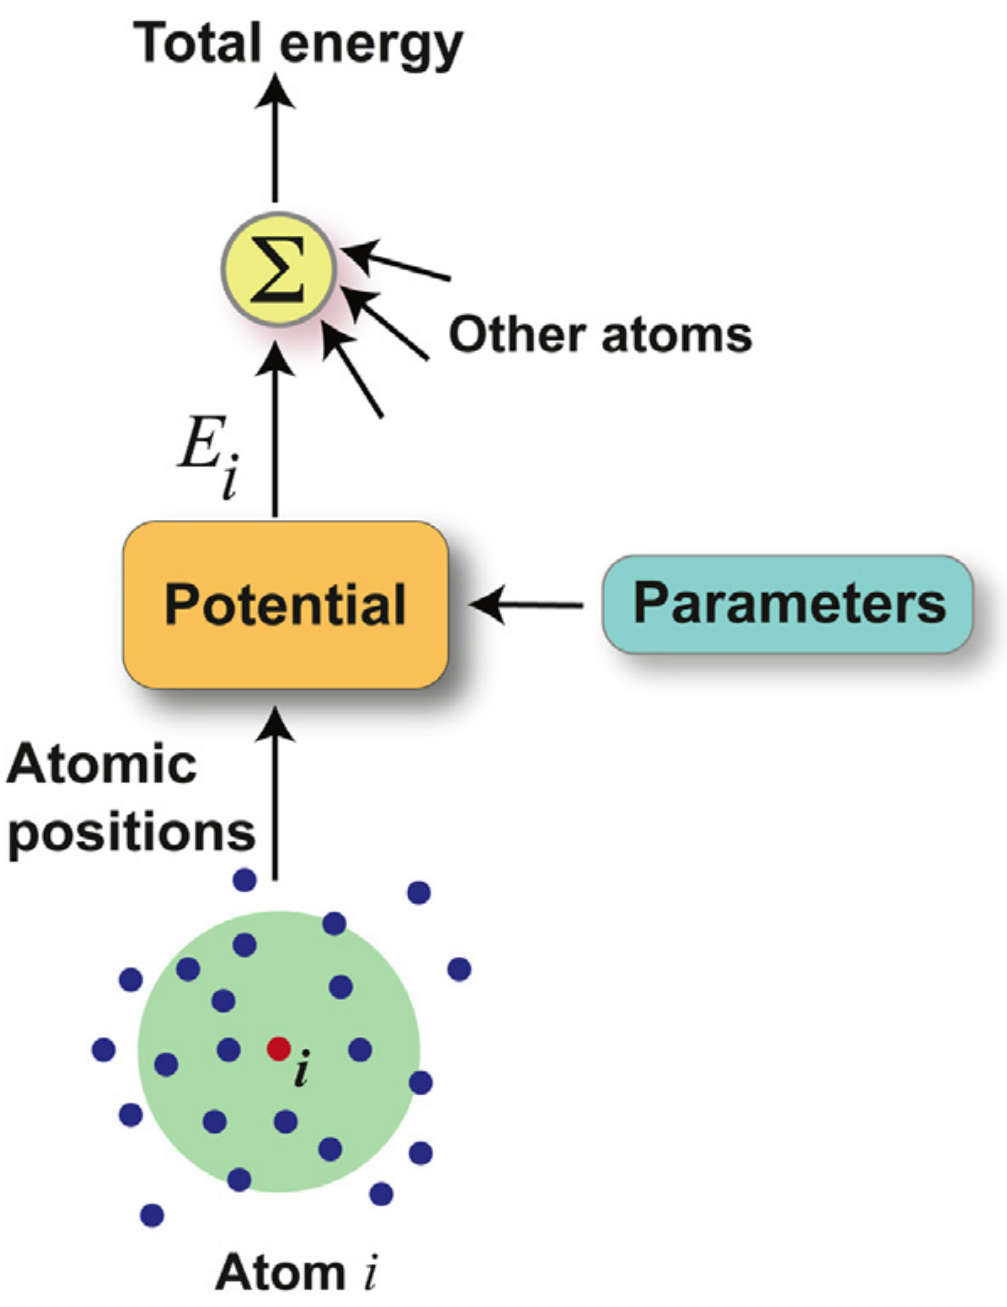
\includegraphics[width=0.5\columnwidth]{intro-ff.png}
            \end{center}
            \column{0.5\textwidth}
            \begin{center}
                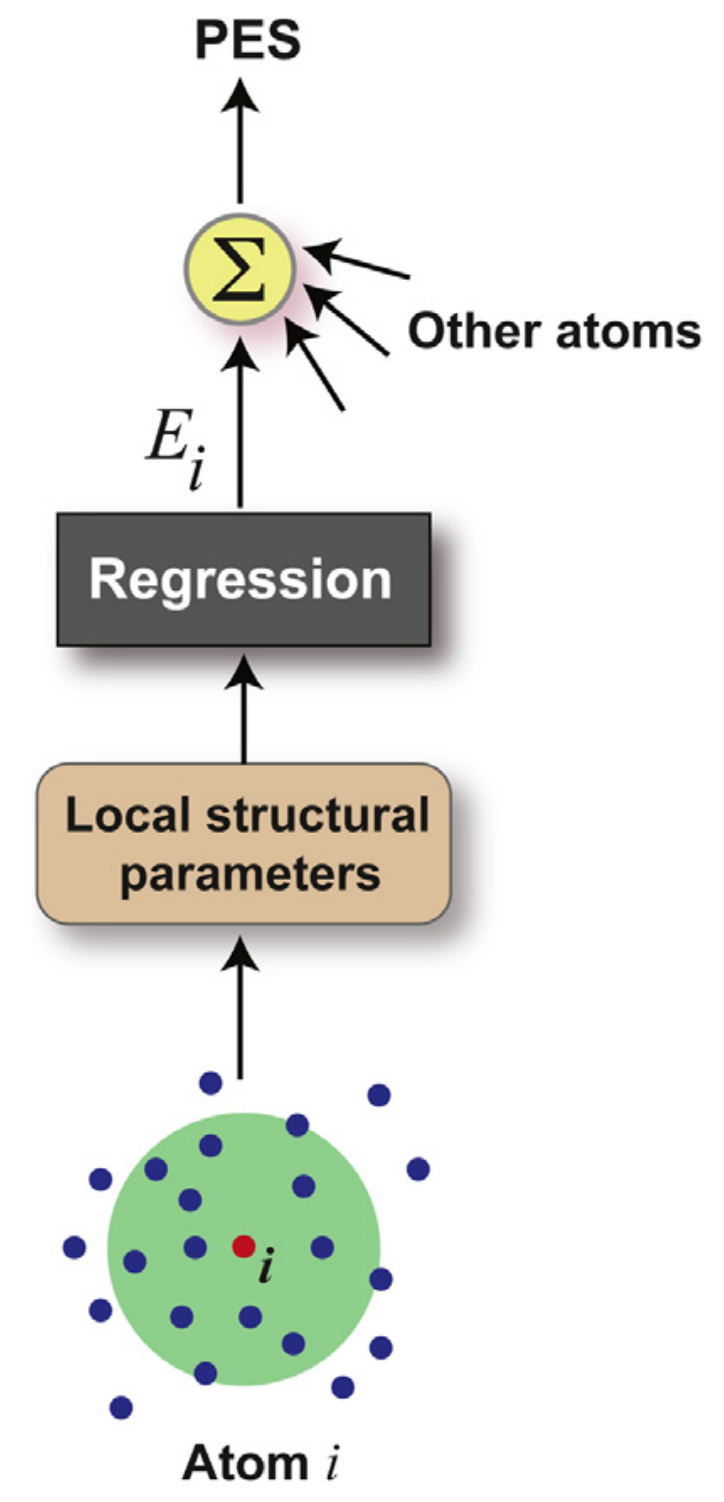
\includegraphics[width=0.3\columnwidth]{intro-ml.png}
            \end{center}
        \end{columns}

        \ \pause

        Existen muchos más descriptores y métodos de ML que se utilizan en el 
        area de trabajo, en este seminario se presentarán sólo algunos de ellos
        que fueron relevantes en el estudio de baterias de litio.

	\end{frame}

    %%%% MÉTODOS %%%%
    \section{Métodos}

    \begin{frame}
        \frametitle{Métodos}
    \end{frame}

    \subsection{Descriptores}
    \begin{frame}
        \frametitle{Métodos: Descriptores}
    \end{frame}

    \subsection{Distintos potenciales de ML}
    \begin{frame}
        \frametitle{Métodos: Distintos potenciales de ML}
    \end{frame}

    %%%% APLICACIONES %%%%
    \section{Aplicaciones en baterias de litio}

    \begin{frame}
        \frametitle{Aplicaciones en baterias de litio}
    \end{frame}

    \subsection{Li$_3$PO$_4$}
    \subsection{LiC}
    \subsection{Li$_x$Si}
    
    %%%% CONCLUSIONES %%%%
    \section{Conclusiones}

    \begin{frame}
        \frametitle{Conclusiones}
    \end{frame}

\end{document}
